\renewcommand{\thechapter}{\roman{chapter}}
\setcounter{chapter}{3}
\setcounter{figure}{0}

\unchapter{Préambule microscopie confocale par réflectance}
\label{chap:preamble_microscopy}
La précédente partie de ce travail consacrée au contexte, permet une mise en situation des connaissances mobilisées pour ce travail et une présentation des recherches liés à celui-ci. Au sein de cette seconde partie est élaborée une méthodologie destinée à la modalité \gls{rcm}. Les éléments nous ayant conduits à nous intéresser à cette modalité sont multiples. En premier lieu, il s'agit de l'une des modalités les plus précises en notre possession, elle consiste donc en une référence en terme de qualité de diagnostic à réaliser. Enfin, le nombre restreint de travaux menés sur le diagnostic de lésion de la peau appliqué au \gls{rcm} assisté par ordinateur est un second argument. En effet, cette modalité représente pour nous un verrou scientifique que nous devons lever pour accomplir le schéma de diagnostic multimodal. Ce préambule a pour objectif de présenter d'une part les données de travail exclusives à la modalité \gls{rcm} introduites lors du \Cref{chap:chapter_31}, et d'autre part de présenter les résultats des experts qui constituent la finalité des méthodes d'aide au diagnostic de cette partie.\par

Ainsi dans cette partie, seules les données \gls{rcm} des 223 lésions en notre possession sont considérées \textbf{pour l'évaluation} des méthodes et sont exclues les images de photographie clinique et de dermatoscopie. Pour rappel, ces données correspondent à des lésions pouvant porter à confusion lors du diagnostic de \gls{lm} et de \gls{lmm} par le spécialiste. En addition à ces données, 28 patients bénins non présents dans la base d'images initiale sont utilisés afin d'augmenter le nombre d'images annotées comme bénignes \textbf{pour l'entraînement} des méthodes développées.\par

Chaque lésion contient des images \gls{rcm} jugées pertinentes par deux des trois médecins investigateurs dont l'acquisition des images provient de la \gls{dej}. En effet, ces deux pathologies sont observables à ce niveau de profondeur~:
\begin{itemize}
    \item les \textbf{pathologies de \gls{lm}} résultent d'une prolifération de cellules au niveau de la lame basale (extrémité supérieure de la \gls{dej}),
    \item les \textbf{pathologies de \gls{lmm}} résultent de l'intrusion de la mélanine se propageant le long des follicules pileux (extrémité supérieure et intérieur de la \gls{dej}).
\end{itemize} Ces images dont l'acquisition est réalisée au niveau de la \gls{dej} sont donc ainsi parfaitement adaptées à la caractérisation de ce phénomène par les médecins.\par

Du point de vue des caractéristiques, ces images arborent une taille constante de \SI{1000}{\px} $\times$ \SI{1000}{\px} pour une section mesurée de \SI{920}{\micro\metre} $\times$ \SI{920}{\micro\metre} pour une résolution en profondeur comprise entre \SIrange{3}{5}{\micro\metre}. Ces données fournissent ainsi une résolution de l'ordre du \SI{1}{\micro\metre}. Les informations d'acquisition (profondeur, longueur d'onde, \ldots) contenues dans les images ne pourront être utilisées car non exploitables (procédure de calibration non réalisée, informations manquantes, \ldots).\par
\clearpage

A partir de ces données, les 18 experts en \gls{rcm} de l'étude~\cite{Cinotti2018} ont obtenu en moyenne une sensibilité de 0,84$\pm$0,05 et une spécificité de 0,75$\pm$0,06 sur l'évaluation des pathologies malignes toutes confondues. Sur l'évaluation des données de \gls{lm} et \gls{lmm}, ces scores deviennent plus homogènes avec une valeur de sensibilité de 0,80$\pm$0,07 et de spécificité de 0.81$\pm$0,05. Les courbes \gls{roc} associées à ces performances sont représentées sur la \Cref{fig:results_roc_rcm_experts}.\par

\begin{figure}[H]
    \begin{center}
        \includegraphics[width=\linewidth]{contents/ii_preamble_microscopy/resources/results_roc_rcm_experts.pdf}
        \caption{Courbes \gls{roc} issues de l'évaluation des données \gls{rcm} par les 18 experts~\cite{Cinotti2018}. A gauche, le résultat des experts mené sur la détection d'éléments malins ; A droite, le résultat des experts mené sur la détection de \gls{lm} et \gls{lmm}.}
        \label{fig:results_roc_rcm_experts}
    \end{center} 
\end{figure}\par

L'objectif visé par cette partie sera d'égaler ces scores à l'aide de nos méthodes de diagnostic sur base d'images issues de \gls{rcm}. A ce titre, nous n'exploiterons pas les méta-données issues des informations patient bien que utilisées par les spécialistes lors de l'évaluation. Ainsi, l'âge, le sexe ou encore l'emplacement sont autant de critères que nous ne considérerons pas au sein de ces prochains paragraphes bien que employés par les dermatologues experts en \gls{rcm} durant leur évaluation. De plus, contrairement aux connaissances des experts, ces méta-données ne sont pas représentatives de la population réelle, et biaiseraient nos méthodes par des corrélations non valides dans le monde réel dû à l'acquisition de la base de données.\par

Ainsi, nous sollicitons diverses ressources d'intelligence artificielle évoquées lors du \Cref{chap:chapter_3}. Des apports ont été réalisés pour permettre le déroulement des expériences que nous présenterons lors des chapitres suivants. En effet, la base d'images actuelle ne possède que des annotations au niveau des patients, ce qui limite fortement nos travaux essentiellement basés sur de l'apprentissage supervisé. A l'aide d'un outil graphique réalisé pour cette étude (\Cref{fig:example_gui_annotation}), nous avons pu obtenir grâce au travail de l'un des dermatologistes investigateur divers niveaux d'annotations supplémentaires, dont~:
\begin{itemize}
    \item des annotations au \textbf{niveau des images} correspondant au plus petit niveau issue des données natives,
    \item des annotations au \textbf{niveau de sous-parties d'images} également appelés \textit{patchs} correspondant à l'extraction d'un nouveau niveau de données à partir des images.
\end{itemize}\par
\clearpage

\begin{figure}[H]
\centering
    \begin{subfigure}{.45\textwidth}
      \centering
      \includegraphics[width=\linewidth]{contents/ii_preamble_microscopy/resources/example_gui_annotation_1.png}
    \end{subfigure}
    \begin{subfigure}{.45\textwidth}
      \centering
      \includegraphics[width=\linewidth]{contents/ii_preamble_microscopy/resources/example_gui_annotation_2.png}
    \end{subfigure}
    \caption{Interface logicielle mise à disposition du spécialiste, afin de procéder aux annotations au niveau des images et des sous-images. A gauche, l'onglet permettant l'annotation au niveau des images ; A droite, l'onglet permettant la création et l'annotation de sous-images.}
    \label{fig:example_gui_annotation}
\end{figure}

Les annotations au niveau des lésions bien que initialement sur deux classes, donnent naturellement lieu au niveau des images à des annotations sur \textbf{trois classes}. Ces annotations sont les suivantes~:
\begin{itemize}
    \item Un premier type d'annotation du nom de \textit{malin} a été apposée \textit{sur des images} contenant \textbf{au moins} du tissu de type malin et \textit{sur des sous-images} contenant essentiellement ce type de tissus. 
    \item Un second type d'annotation du nom de \textit{bénin} a été apposé \textit{sur des images} ne contenant \textbf{aucun} tissus malin mais \textbf{au moins} du tissu bénin et \textit{sur des sous-images} composées de ce type de tissus. 
    \item  Enfin, un troisième type d'annotation du nom \textit{sain} a été renseignée \textit{sur des images} ne contenant \textbf{aucun} des deux types de tissus précédents et \textit{sur des sous-images} composées de tissus sains. 
\end{itemize} Des exemples de ces images et diverses annotations sont visibles sur la \Cref{fig:example_rcm_data}.\par

La répartition complète de cette base annotée peut être visualisée sur la \Cref{fig:scheme_rcm_statistics}. Nous pouvons y visualiser la composition de la base d'image et celle des sous-images ou patchs. La couleur bleu permet de visualiser le jeu de données initial servant à l'entraînement et l'évaluation~\cite{Cinotti2018}, et en orange les données servant à corriger partiellement le non balancement lors de l'entraînement.\par

\begin{figure}[H]
    \begin{center}
        \includegraphics[width=\linewidth]{contents/ii_preamble_microscopy/resources/example_rcm_data.pdf}
        \caption{Exemple de tissus et annotations, considérés respectivement de gauche à droite comme \textit{sain}, \textit{bénin} et \textit{malin} par le spécialiste.}
        \label{fig:example_rcm_data}
    \end{center} 
\end{figure}\par

\begin{figure}[H]
    \begin{center}
        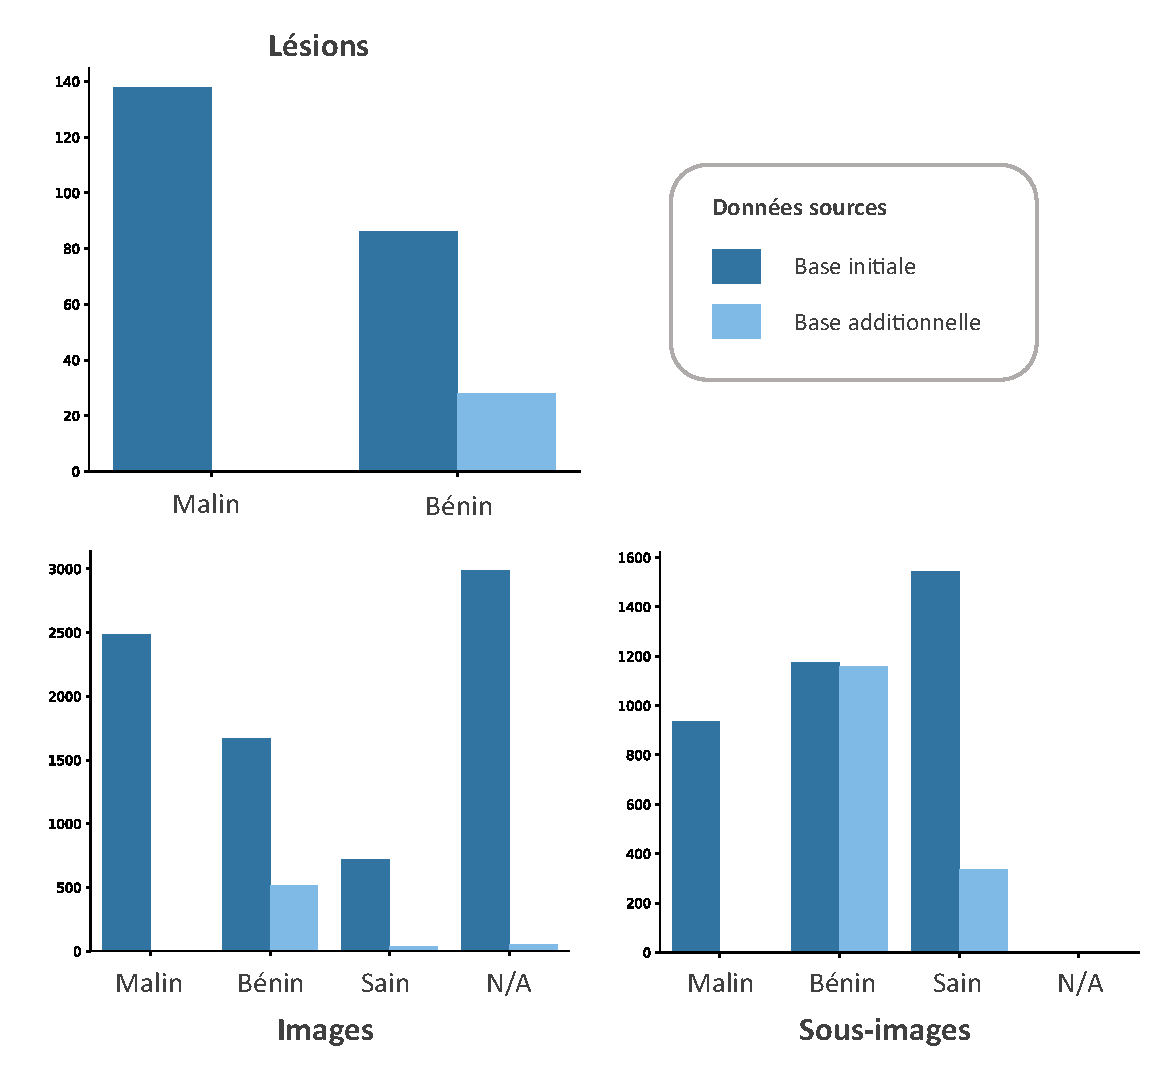
\includegraphics[width=\linewidth]{contents/ii_preamble_microscopy/resources/scheme_rcm_statistics.pdf}
        \caption{Répartition des annotations réalisées par l'expert, en bleu sur la base initiale de Cinotti~\cite{Cinotti2018} et en orange sur les données bénignes supplémentaires. A gauche, la répartition des annotations images ; A droite, la répartition des annotations sur les sous-images.}
        \label{fig:scheme_rcm_statistics}
    \end{center} 
\end{figure}\par

Afin de répondre à ce besoin de diagnostic au niveau des lésions acquises par \gls{rcm}, cette partie dédiée à cette modalité se compose de trois chapitres dans lesquels est développée une méthodologie ascendante~:
\begin{itemize}
    \item dans un premier temps, le \Cref{chap:chapter_4} aborde la \textbf{prise de décision au niveau de l'image} par des schémas simples permettant une prise de décision sur les images \gls{rcm},
    \item dans un second temps, le \Cref{chap:chapter_5} propose des méthodes destinées à \textbf{améliorer ce diagnostic image} par la mise en oeuvre de schémas avancés permettant à nouveau la prise de décision sur les images \gls{rcm},
    \item enfin, le \Cref{chap:chapter_6} se focalise sur une \textbf{prise de diagnostic au niveau du patient} par la présentation de processus décisionnel au niveau lésionnel.
\end{itemize}\par
\newpage